

\documentclass[ border=0pt, a4paper, 11pt]{article}
\usepackage[left=2cm,right=2cm,top=2cm,bottom=2cm]{geometry}
\usepackage[utf8]{inputenc}
\usepackage{graphicx,amsmath,amsfonts,amssymb}
\usepackage{tikz}
\usepackage{fancyhdr}
\pagestyle{fancy}
\usetikzlibrary{positioning, shapes}
\usepackage{xcolor}

\pgfdeclarelayer{background}
\pgfdeclarelayer{foreground}
\pgfsetlayers{background,main,foreground}
\definecolor{pprime1}{RGB}{89,167,167}
\definecolor{pprime2}{RGB}{45,164,170}
\definecolor{pprime3}{RGB}{82,162,161}
\definecolor{brown}{RGB}{165,42,42}
\renewcommand{\headrulewidth}{0pt}
\usepackage{transparent}
\usetikzlibrary{patterns}

\numberwithin{equation}{section}
\newcommand{\Rho}{\textcolor{violet}{\rho'}}
\renewcommand{\u}{\textcolor{red}{u'}}
\renewcommand{\v}{\textcolor{green}{v'}}
\newcommand{\w}{\textcolor{blue}{w'}}
\newcommand{\p}{\textcolor{cyan}{p'}}
\newcommand{\T}{\textcolor{pink}{T'}}
\newcommand{\Mu}{\textcolor{magenta}{\mu'}}
\newcommand{\Kappa}{\textcolor{yellow}{\kappa'}}

\begin{document}
%%%%%%%%%%%%%%%%%%%%%%%%%%%%%%%%%%%%%%%%%%%%%%%%%%%%%%%%%%%%%%%%%%%%%%%%%%%%%%%%%%%%%%%%%%%%%%%%%%%%%%%%%%%%%%%%%%%



\section{Sparse Matrix definition and calculation optimization}

To avoid memory saturation during the resolution of eigenvalue problem it is necessary to write sparse matrix with the sparse method possible in Matlab. I base my programming upgrades based on the Trefethen' book "Spectral Methods in Matlab", page 93-95 program 23. The problem described in this exercise is :
\begin{equation}
   \Delta u = e^{20(y-x-1)}
\end{equation}



\subsection{ Definition of$ (A- \lambda B) $ }

The objective is to obtain a $(Nx*Ny*Neq)^2$ Matrix with Nx = 2000, Ny = 200, Neq = 7. But writing such matrix is beyond computer memory capacity (16 Gb).
Therefore one wants to write all matrices without writing any zero from the very begin of the code. 
I calculated that for $\Delta u =0$ problem at :\\
Nx = Ny = 20 \& Neq = 1, Matrix is $90\%$ zero elements\\
Nx = Ny = 200 \& Neq = 1, Matrix is $99\%$ zero elements\\

It can be expected that for Nx = 2000, Ny = 200, Neq = 7, Matrix should be $95\%$ zero.
In this case, this a $5\%$ non zero elements matrix as estimated, it could be stored in the memory.
The only matrices that are written as Matrix elements (not sparse elements) are Chebyshev matrix $D$ and Chebyshev square $D2$ that are only $(Nx*Ny)^2$ .

For now, with non fully sparse method I reached N = 200 before memory saturation while I need to reach at least Nx = Ny = 1700 for Neq =1 .


\subsection{ Eigenvalues and Eigenvectors}
Here we can see the results of the Laplacian problem with perturbation :\\
\begin{tabular}{cc}
   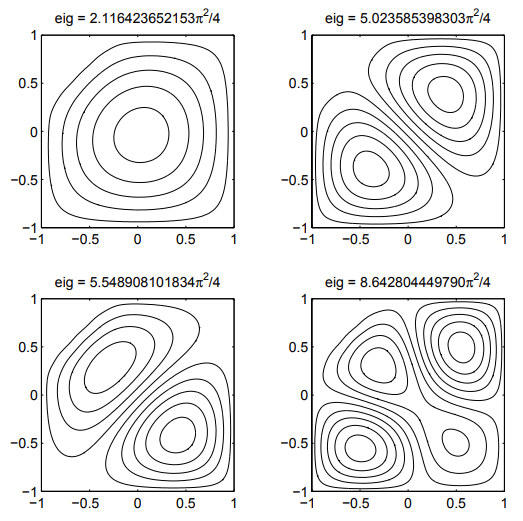
\includegraphics[width=8cm]{eigenvalue_perrtub.PNG} &
   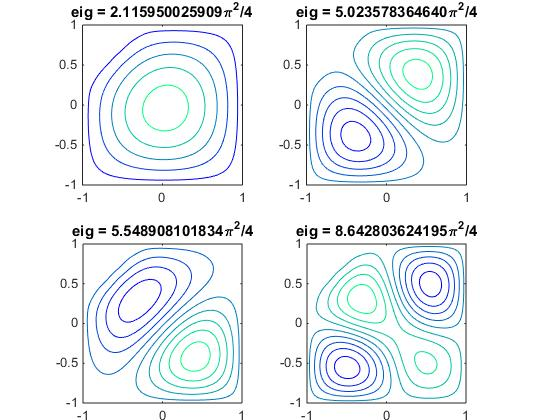
\includegraphics[width=10.5cm]{eigenvalue_sparse.jpg} \\
\end{tabular}\\
On the right side, one can see the results from Trefethen's book , on the left our results with the new sparse method.
The average error between the two methods for eigenvalues is less than $10^{-11}$. It is negligible.

Time of calculation is expected to be divided by 300-400 with the new sparsing method compared to eig resolution method and twice quicker than non sparse method.

In this annex there is the full code to solve the example. Subsection "D2X full sparsing method" is equivalent to $\frac{\partial^2 .}{\partial x^2}$ and "D2Y full sparsing method" is equivalent to $\frac{\partial^2 .}{\partial y^2}$. The sum on those sections is a Laplacian. Those sections describe the way to write a sparse matrix from the beginning with "triple vector".


\section{annex}




\begin{equation}
 \rho\frac{\partial \u }{\partial x} + \rho\frac{\partial \v }{\partial y} + \rho\frac{\partial \w }{\partial z} + \rho\frac{\partial u_o}{\partial x} + \rho\frac{\partial v_o}{\partial y}  =0
\end{equation}

\begin{multline}
\\\rho \frac{\partial \u }{\partial t} + \rho \u \frac{\partial u_o}{\partial x} + \rho u_o\frac{\partial \u }{\partial x} + \rho \u \frac{\partial v_o}{\partial y} + \rho v_o\frac{\partial \u }{\partial y} + \rho w_o\frac{\partial \u }{\partial z}\\ + \rho u_o\frac{\partial \u }{\partial x} + \rho \u \frac{\partial u_o}{\partial x} + \rho u_o\frac{\partial \v }{\partial y} + \rho \v \frac{\partial u_o}{\partial y} + \rho u_o\frac{\partial \w }{\partial z}
\\=-\frac{\partial \p }{\partial x} +  \frac{\partial \mu_o}{\partial x}  \frac{\partial \u }{\partial x} + \frac{\partial \mu_o}{\partial x} \frac{\partial \u }{\partial x} + \left(- \frac{2}{3}\frac{\partial\mu_o }{\partial x}\frac{\partial \u }{\partial x}\right) + \left(-\frac{2}{3}\frac{\partial\mu_o }{\partial x}\frac{\partial \v }{\partial y}\right) + \left(-\frac{2}{3}\frac{\partial\mu_o }{\partial x}\frac{\partial \w }{\partial z} \right)\\ +  \frac{\partial \mu_o}{\partial x}  \frac{\partial \v }{\partial x} + \frac{\partial \mu_o}{\partial x} \frac{\partial \u }{\partial y}  +  \frac{\partial \mu_o}{\partial x}  \frac{\partial \w }{\partial x} + \frac{\partial \mu_o}{\partial x} \frac{\partial \u }{\partial z} \\ +  \frac{\partial  \Mu }{\partial x}  \frac{\partial u_o}{\partial x} + \frac{\partial  \Mu }{\partial x} \frac{\partial u_o}{\partial x} + \left[-\frac{\partial \Mu  }{\partial x}\frac{2}{3}\left(                \frac{\partial u_o}{\partial x}+\frac{\partial v_o}{\partial y}                 \right)\right] +  \frac{\partial  \Mu }{\partial x}  \frac{\partial v_o}{\partial x} + \frac{\partial  \Mu }{\partial x} \frac{\partial u_o}{\partial y}  + \frac{\partial  \Mu }{\partial x} \frac{\partial w_o}{\partial x} \\ + \mu_o \frac{\partial^2 \u  }{\partial x^2} + \mu_o \frac{\partial^2 \u  }{\partial x \partial x } + \left(-\frac{2\mu_o }{3}\frac{\partial^2 \u }{\partial x^2}\right) + \left(-\frac{2\mu_o}{3}\frac{\partial^2 \v }{\partial x\partial y}\right) + \left(-\frac{2\mu_o}{3}\frac{\partial^2 \w }{\partial x\partial z}\right) + \mu_o \frac{\partial^2 \v  }{\partial x^2} + \mu_o \frac{\partial^2 \u  }{\partial x \partial y } + \mu_o \frac{\partial^2 \w  }{\partial x^2} + \mu_o \frac{\partial^2 \u  }{\partial x \partial z }\\ +  \Mu  \frac{\partial^2 u_o }{\partial x^2} +  \Mu  \frac{\partial^2 u_o }{\partial x \partial x } + \left[-\frac{2 \Mu  }{3}\frac{\partial}{\partial x}\left(                \frac{\partial u_o}{\partial x}+\frac{\partial v_o}{\partial y}                 \right)\right] +  \Mu  \frac{\partial^2 v_o }{\partial x^2} +  \Mu  \frac{\partial^2 u_o }{\partial x \partial y } +  \Mu  \frac{\partial^2 w_o }{\partial x^2}\\\right) \frac{1}{Re} 
\end{multline}

\begin{multline}
\\\rho \frac{\partial \u }{\partial t} + \rho \u \frac{\partial u_o}{\partial x} + \rho u_o\frac{\partial \u }{\partial x} + \rho \u \frac{\partial v_o}{\partial y} + \rho v_o\frac{\partial \u }{\partial y} + \rho w_o\frac{\partial \u }{\partial z}\\ + \rho u_o\frac{\partial \u }{\partial x} + \rho \u \frac{\partial u_o}{\partial x} + \rho u_o\frac{\partial \v }{\partial y} + \rho \v \frac{\partial u_o}{\partial y} + \rho u_o\frac{\partial \w }{\partial z}
\\=-\frac{\partial \p }{\partial x} +  \frac{\partial \mu_o}{\partial x}  \frac{\partial \u }{\partial x} + \frac{\partial \mu_o}{\partial x} \frac{\partial \u }{\partial x} + \left(- \frac{2}{3}\frac{\partial\mu_o }{\partial x}\frac{\partial \u }{\partial x}\right) + \left(-\frac{2}{3}\frac{\partial\mu_o }{\partial x}\frac{\partial \v }{\partial y}\right) + \left(-\frac{2}{3}\frac{\partial\mu_o }{\partial x}\frac{\partial \w }{\partial z} \right)\\ +  \frac{\partial \mu_o}{\partial x}  \frac{\partial \v }{\partial x} + \frac{\partial \mu_o}{\partial x} \frac{\partial \u }{\partial y}  +  \frac{\partial \mu_o}{\partial x}  \frac{\partial \w }{\partial x} + \frac{\partial \mu_o}{\partial x} \frac{\partial \u }{\partial z} \\ +  \frac{\partial  \Mu }{\partial x}  \frac{\partial u_o}{\partial x} + \frac{\partial  \Mu }{\partial x} \frac{\partial u_o}{\partial x} + \left[-\frac{\partial \Mu  }{\partial x}\frac{2}{3}\left(                \frac{\partial u_o}{\partial x}+\frac{\partial v_o}{\partial y}                 \right)\right] +  \frac{\partial  \Mu }{\partial x}  \frac{\partial v_o}{\partial x} + \frac{\partial  \Mu }{\partial x} \frac{\partial u_o}{\partial y}  + \frac{\partial  \Mu }{\partial x} \frac{\partial w_o}{\partial x} \\ + \mu_o \frac{\partial^2 \u  }{\partial x^2} + \mu_o \frac{\partial^2 \u  }{\partial x \partial x } + \left(-\frac{2\mu_o }{3}\frac{\partial^2 \u }{\partial x^2}\right) + \left(-\frac{2\mu_o}{3}\frac{\partial^2 \v }{\partial x\partial y}\right) + \left(-\frac{2\mu_o}{3}\frac{\partial^2 \w }{\partial x\partial z}\right) + \mu_o \frac{\partial^2 \v  }{\partial x^2} + \mu_o \frac{\partial^2 \u  }{\partial x \partial y } + \mu_o \frac{\partial^2 \w  }{\partial x^2} + \mu_o \frac{\partial^2 \u  }{\partial x \partial z }\\ +  \Mu  \frac{\partial^2 u_o }{\partial x^2} +  \Mu  \frac{\partial^2 u_o }{\partial x \partial x } + \left[-\frac{2 \Mu  }{3}\frac{\partial}{\partial x}\left(                \frac{\partial u_o}{\partial x}+\frac{\partial v_o}{\partial y}                 \right)\right] +  \Mu  \frac{\partial^2 v_o }{\partial x^2} +  \Mu  \frac{\partial^2 u_o }{\partial x \partial y } +  \Mu  \frac{\partial^2 w_o }{\partial x^2}\\\right) \frac{1}{Re} 
\end{multline}

% Program 23 of Trefethen book page 93-95
clear all;
N = 16 ;

%% cheb function
x = cos(pi*(0:N)/N)';
c = [2; ones(N-1,1); 2].*(-1).^(0:N)';
X = repmat(x,1,N+1);
dX = X-X';
cheb  = (c*(1./c)')./(dX+(eye(N+1)));      % off-diagonal entries
cheb  = cheb - diag(sum(cheb'));
%% mesh

y = x;
[xx,yy] = meshgrid(x(2:N),y(2:N)) ;
xx = xx(:) ; yy = yy(:) ;

%% D²
D2 = cheb^2 ; D2 = D2(2:N,2:N) ;

%%  D2X full sparsing method
    for n = 1:(N-1)^2
            [row,col] = ind2sub(size(D2),n);
            D2X(n,1) = row ;
            D2X(n,2) = col;
            D2X(n,3) = D2(row,col);
    end
 for n = 1:N-1 
    D2X(1+(n-1)*(N-1)^2:n*(N-1)^2,1) = D2X(1:(N-1)^2,1) + (N-1)*(n-1);
    D2X(1+(n-1)*(N-1)^2:n*(N-1)^2,2) = D2X(1:(N-1)^2,2) + (N-1)*(n-1);
    D2X(1+(n-1)*(N-1)^2:n*(N-1)^2,3) = D2X(1:(N-1)^2,3); 
 end 
 D2X = sparse(D2X(:,1),D2X(:,2),D2X(:,3));  

 %% D2Y full sparsing method
   D2Y=zeros((N-1)^3,3);
    for n = 1:(N-1)^2
    [row,col] = ind2sub(size(D2),n);        
    D2Y((n-1)*(N-1)+1:n*(N-1),1)= (row-1)*(N-1)+(1:N-1);
    D2Y((n-1)*(N-1)+1:n*(N-1),2)= (col-1)*(N-1)+(1:N-1);
    D2Y((n-1)*(N-1)+1:n*(N-1),3)= D2(row,col);
    end
    D2Y = sparse(D2Y(:,1),D2Y(:,2),D2Y(:,3));
    
 %% definition of L   laplacian = exp(20*(y-x-1)
    L = -D2X -D2Y ; 
    H = sparse(diag(exp(20*(yy-xx-1))));
    L = L + H;
    
 %% Reslolution   
    [V,D] = eigs(L,N,5.548908101834*pi^2/4); 
    % the value is given page 94  Specral Methods in Matlab, by Lloyd N. Trefethen as an example
    
    %eigenvalues
    D = diag(D) ;
    [D,ii] = sort(D) ;
    ii = ii(1:4); 
    %eigenvectors
    V = V(:,ii);
    
    %% finer meshing for plot
    [xx,yy] = meshgrid(x,y) ;
    [X,Y] = meshgrid(-1:.02:1,-1:.02:1);
    uu = zeros(N+1,N+1) ;
    [ay,ax] = meshgrid([.56 .04],[.1 .5]);

    %% plot 
    figure(2)
    for i= 1:4
        uu(2:N,2:N) = reshape(V(:,i),N-1,N-1) ;
        uu = uu/norm(uu(:),inf);
        U = interp2(xx,yy,uu,X,Y,'cubic');
        subplot('position',[ax(i) ay(i) .38 .38])
        contour(-1:.02:1,-1:.02:1,U,-.9:.2:.9) %eigenvectors plot
        colormap(winter), axis square
        title(['eig = ' num2str(D(i)/(pi^2/4),'%18.12f') '\pi^2/4']) %eigenvalue writing
    end
    \v
\end{document}